\documentclass[12pt, a4paper, oneside]{ctexart}
\usepackage{amsmath, amsthm, amssymb, graphicx, fancyhdr, pinyin}
\pagestyle{fancy}
\title{非甾体抗炎药的合理使用与开发}
\author{生信 2001 张子栋\thanks{E-mail: zidongzh@outlook.com}}
% 去掉日期
\date{}
% 页眉
\lhead{华中农业大学}
\rhead{药物化学结课论文}

% 正文部分
\begin{document}

\maketitle
\thispagestyle{empty}
\newpage

\tableofcontents

\thispagestyle{empty}
\setcounter{page}{0}

\newpage

% 摘要部分
\begin{abstract}
    非甾体抗炎药是生活中较为常用、适应症多的一种药物,
    通常用于消炎、止疼(如布洛芬缓释胶囊)和退热(如扑热息痛(对乙酰氨基酚))。
    另外在施用剂量较大时也有抗血栓作用。
    此类药物的副作用也十分明显,因此不宜长期服用或同类药物联用。
    目前此类药物已经十分成熟,新药研制方面也有许多不同的方向。
\end{abstract}

\textbf{关键字:}非甾体抗炎药、止疼、炎症、环氧化酶

\newpage
\section{非甾体抗炎药的定义}
\subsection{非甾体抗炎药的分类}
非甾体抗炎药可以通过多种方法分类。
由于其直接作用于环氧化酶,可以通过是否特异性作用于环氧化酶 II 
将其分为非选择性非甾体抗炎药和选择性非甾体抗炎药。
从化学本质上分类,可分为多氨基酚类、水杨酸类、烯醇酸类、乙酸类、吡唑酮类、昔布类。

\subsection{非甾体抗炎药的性质}
\subsubsection{甾体与非甾体抗炎药}
甾 ({\zai1}) 体也译作类固醇 (steroid) 或糖皮质激素。译作这个生僻字「甾」并不是中国科学家故作高深,
建起学术壁垒,反而体现了汉字作为象形字的魅力,「巛」代表了侧链,「田」代表了四个环\cite{ref1}。
如下图 1\footnote{Guillem d'Occam - CC BY-SA 3.0},胆固醇也是一种甾体。

\begin{figure}[htbp]
    \centering
    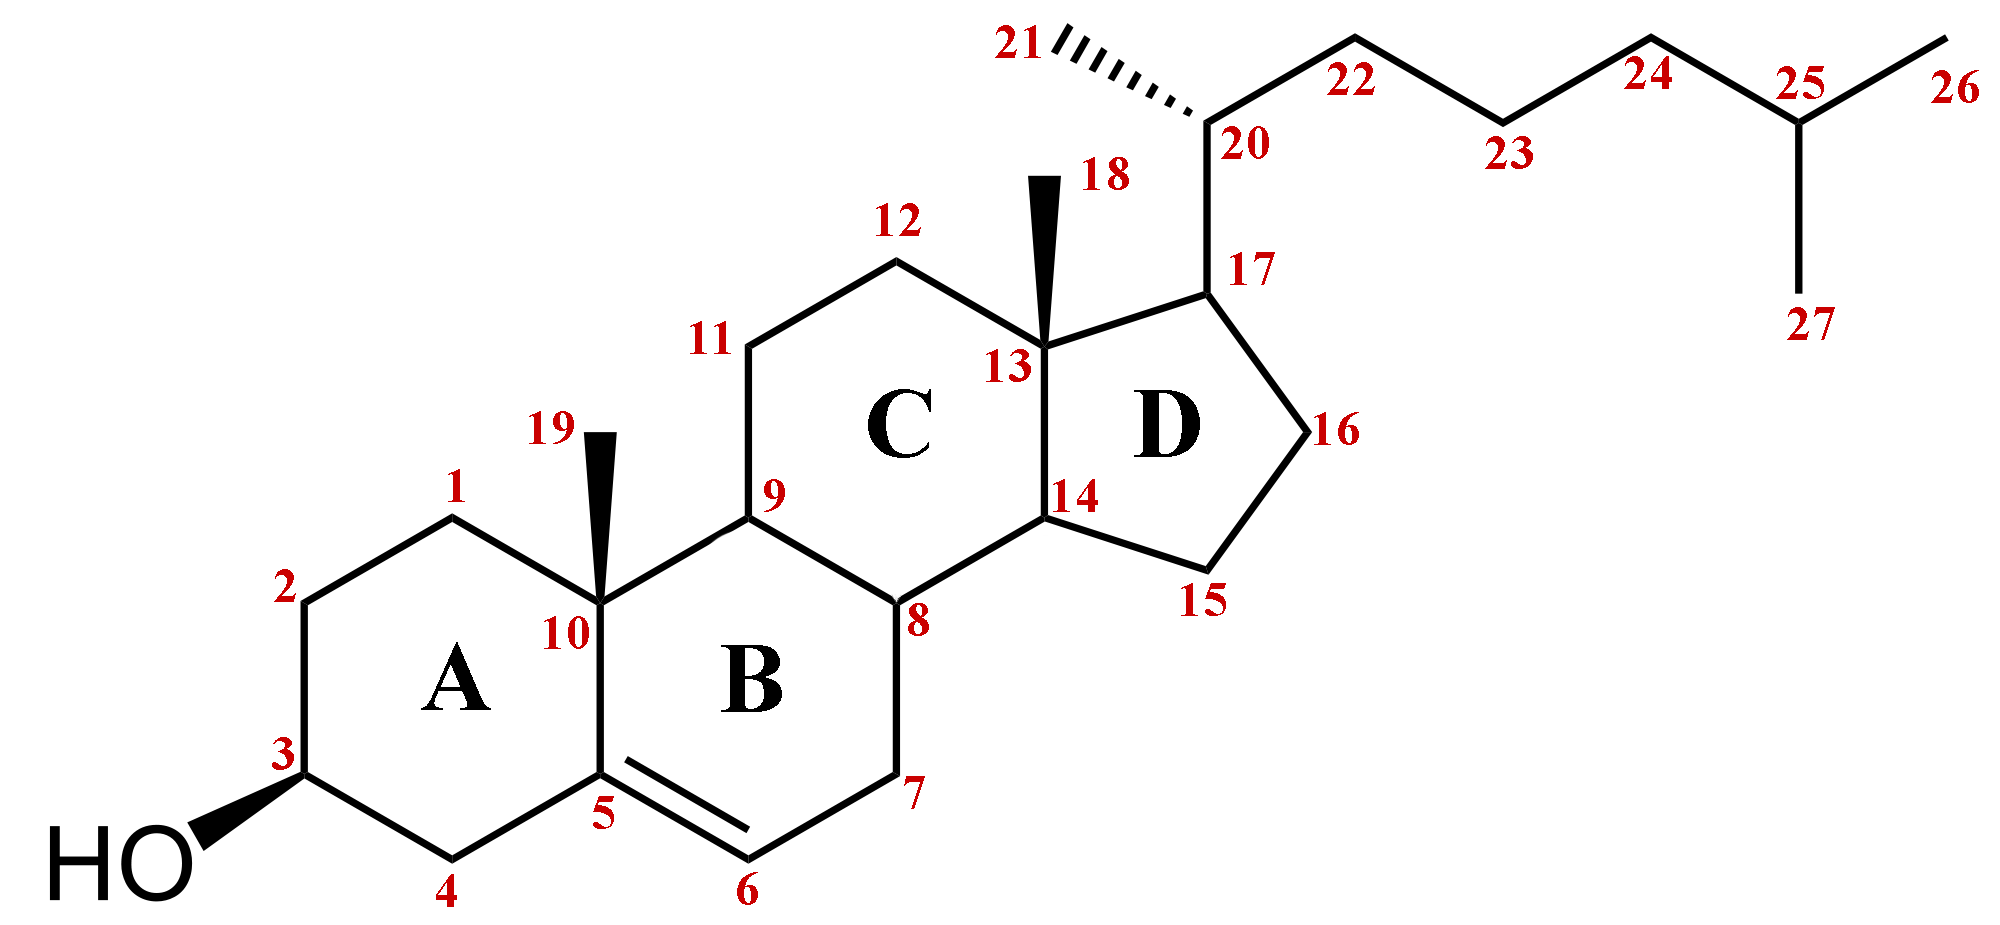
\includegraphics[width=10cm,height=4.625cm]{Colesterol.png}
    \caption{胆固醇 Colesterol}
    \end{figure} 

甾体在生物体内主要作为激素,甾体类药物具有很强的消炎和免疫抑制作用,但同时也具有很大的副作用。
2003 年在我国爆发的非典疫情中,由于缺乏抗病毒药物,多数重症患者均使用了糖皮质激素进行治疗,
并且治疗效果良好。但在使用糖皮质激素治疗的患者中,均不同程度的出现了股骨头坏死的后遗症,
据研究股骨头坏死与使用大量糖皮质激素有一定关系\cite{ref2}。

由于甾体类药物的副作用较大,新的具有抗炎作用的非甾体药物被研制出来。为了与具有抗炎作用的甾体区分开,
这类药物取名非甾体抗炎药 (Non-Steroidal Anti-Inflammatory Drugs, NSAIDs)。
1952 年保泰松,并开始使用 NSAIDs 这个名称。

\subsection{非甾体抗炎药的历史沿革}
非甾体抗炎药这个名称是在 1952 年开始使用,但是第一种非甾体抗炎药问世的时间要早得多。
很久以前,人们就发现柳树皮具有一定的抗炎解热作用,并在 1838 年成功从柳树皮中提取出水杨酸,
在 1860 年实现了水杨酸的人工合成。之后在 1899 年拜尔公司将水杨酸的酚羟基乙酰化
(如图 2\footnote{By File:Aspirin-skeletal.svg originally by Benjah-bmm27 and Booyabazooka, edited by Fvasconcellos - File:Aspirin-skeletal.svg, Public Domain}),
推出阿司匹林,并迅速成为世界上使用最广泛的药物之一。

\begin{figure}[htbp]
    \centering
    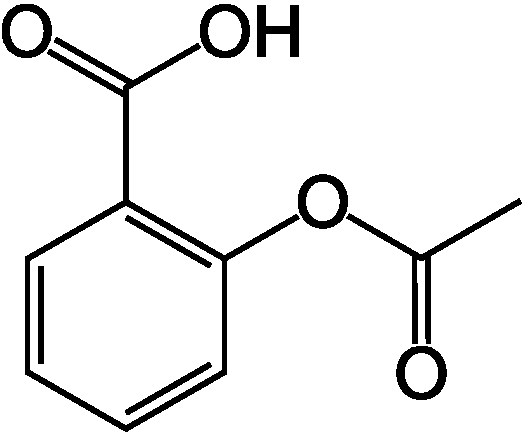
\includegraphics[width=4cm]{Aspirin-skeletal.pdf}
    \caption{阿司匹林 Aspirin}
    \end{figure}

之后还出现了对抗疟药物奎宁进行改造的吡唑酮类药物,但由于其可能引起白细胞减少、粒细胞缺乏
的不良反应,已经被淘汰。

\newpage
\section{非甾体抗炎药的作用及其作用原理}
\subsection{非甾体抗炎药对环氧化酶抑制作用}

\subsection{前列腺素与血栓素的作用}

\subsection{非甾体抗炎药的作用}
\subsubsection{消炎作用}

\subsubsection{止疼作用}

\subsubsection{退热作用}

\subsubsection{抗血栓作用}



\newpage
\section{常见非甾体抗炎药}
\subsection{非选择性非甾体抗炎药}

\subsection{选择性非甾体抗炎药}


\newpage
\section{非甾体抗炎药用药注意事项}
\subsection{与咖啡因联用}

\subsection{非甾体抗炎药对胃黏膜的损伤}


\newpage
\section{非甾体抗炎药的研发方向}
\subsection{选择性非甾体抗炎药}

\subsection{$NO$ 释放型非甾体抗炎药}


\newpage
\section*{致谢}
感谢老师的言传身教,并在课程的结尾给我们一个上台展示的机会,锻炼我们表达能力。

感谢我的女友金诗琪,她在我完成这篇论文期间不离不弃的支持,
让我平淡无奇的学习生活变得五彩斑斓。
精神上的支持好过任何一种非甾体抗炎药。希望我们的未来更加美好。

感谢我的电脑和键盘以及 Leslie Lamport 开发的 \LaTeX \ 排版系统,
它们是我完成这篇论文的重要基础。

感谢陪伴我三年的颈椎病,如果不是因为它,
我也不会没有磕绊地说出「对乙酰氨基酚」「塞来昔布」「盐酸乙哌立松」这种复杂的药名,
更不会深入了解非甾体抗炎药的作用机制。

在今天的中国,优质的高等教育仍是一种及其稀缺的资源。
因此,我必须牢记自己的责任与使命。
希望这篇论文不是学术思考的终点。

\begin{thebibliography}{99}

    \bibitem{ref1}https://zh.wikipedia.org/wiki/甾体
    \bibitem{ref2}王佰亮. 皮质类固醇性股骨头坏死发病机制与早期干预研究[D]. 中国协和医科大学, 2007.
    \bibitem{ref3}
    \bibitem{ref4}
    \bibitem{ref5}
    
\end{thebibliography}


\end{document}